\chapter{Background}\label{cap:estadodelarte}
\hypenation{MapReduce}

\noindent This second chapter tries to acquaint the reader with the key concepts that define Cloud Computing as well as the MapReduce archetype. Later successive elaborations to the project will lay on top of them.


\section{Cloud Computing}\label{sec:computacioncloud}

\noindent In essence, Cloud Computing, or Cloud for short, is a distributed computing model that attempts to ease the consumption on-demand of that distributed infrastructure, by exporting it as virtual computational resources, platforms or services. However it may seem, the Cloud is no new technology but it introduces a new manner to exploit idle computing capacity. What it intends is to make orchestration of enormous data centers more flexible, so as to allow a user to start or destroy virtual machines as required --- Infrastructure as a Service (\emph{IaaS}) ---, leverage a testing environment over a particular Operating System or software platform --- Platform as a Service (\emph{PaaS}) --- or use a specific service like remote backup --- Software as a Service (\emph{SaaS}). Figure \ref{fig:cloudlayers} shows the corresponding high level layer diagram of a generic Cloud.

\begin{figure}[tbp]
\begin{center}
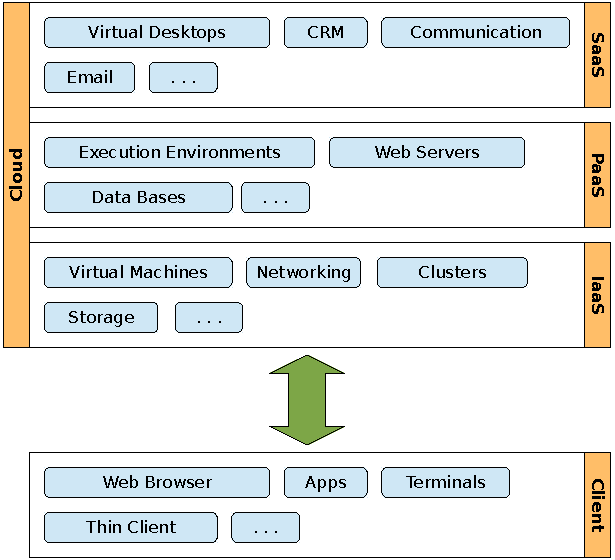
\includegraphics[width=0.69\textwidth]{imagenes/003.pdf}
 \caption{Layers in a cloud in production}
\label{fig:cloudlayers}
\end{center}
\end{figure}

Different IaaS frameworks will cover the functionality that is required to drive the cloud-defining \emph{physical} infrastructure. Nonetheless, an effort to analyze, design, configure, install and maintain the intended service will be needed, bearing in mind that the degree of elaboration grows from IaaS services to SaaS ones. In effect, PaaS and SaaS layers are lied supported by those immediately under --- software is implemented over a particular platform which, in turn, is also build upon a physical layer. Every Cloud Framework focuses on giving the option to configure a stable environment in which to run virtual machines defined by four variables: Virtual CPU count, virtual RAM, virtual persistent memory and virtual networking devices. Such an environment makes it possible to deploy virtual clusters upon which to install platforms or services to be subsequently consumed by users, bringing up the software layers that give form PaaS and SaaS paradigms respectively.

No less important cuestions like access control, execution permissions, quota or persistent or safe storage will also be present in all of the frameworks.


\subsection{Architecture}\label{subsec:arquitecturacloud}

\noindent Figure \ref{fig:cloudlayers} showed possible layers that could be found in a cloud deployment. Depending on the layers that are implemented, the particular framework and the role played by the cluster node, different particular modules will appear to make possible the consumption of configured services. These modules may be though of as Cloud subsystems that connect each one of the parts that are required to execute virtual machines. Those virtual machines' capabilities are defined by the four variables previously discussed --- VCPUS, RAM, HDD and networking. As there is no methodology dictating how those subsystems should be in terms of size and responsibility, and thus, each framework makes its own modular partition regarding infrastructure management.

Setting modularity apart, one common feature among different clouds is the separation of responsibility in two main roles: \emph{Cloud Controller} and \emph{Cloud Node}. Figure \ref{fig:archcloud} shows a generic Cloud deployment in a cluster with both roles defined. The guidelines followed for having this two roles lies close to \emph{Master-Slave} architectures' approach. In those, in the abstract, there's a set of computers labeled as coordinators which are expected to control execution, and another set made up with those machines that are to carry out the actual processing.

\begin{figure}[tbp]
\begin{center}
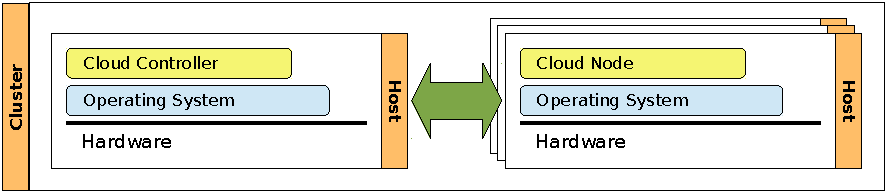
\includegraphics[width=0.9\textwidth]{imagenes/004.pdf}
 \caption{Cloud Controller and Cloud Node}
\label{fig:archcloud}
\end{center}
\end{figure}

Within this general role distribution in a cluster, host computers or cluster nodes --- labeled as Cloud Controllers or Cloud Nodes --- cooperate in a synchronized fashion through \emph{NTP} (\emph{Network Time Protocol}) and communicate via message passing supported by asynchronous queues. To store services' metadata and status they typically draw upon a \emph{DBMS} (\emph{Data Base Management System}) implementation, which is regularly kept running in a dedicated cluster node set sharded (distributed) between the members of the set.

Although there is no practical restriction to configuring both Cloud Controller and Cloud Node within a single computer in a cluster, this approach should be limited to development environments due to the considerable impact in performance that it would carry.


\subsubsection{Cloud Controller}\label{subsubsec:cloudcontroller}

\noindent The fundamental task for a Controller is to maintain all of the cloud's constituent modules working together by coordinating their cooperation. As an example, it is a Controller's duty to:

\begin{itemize}
 \item Authentication and authorization control.
 \item Available infrastructure resources recount.
 \item Quota management.
 \item Usage balance.
 \item User and project inventory.
 \item API exposure for service consumption.
 \item Real time cloud monitoring.
\end{itemize}

Being an essential part of a cloud as it is, the Controller node (not to be mistaken for the Cloud Node) is usually replicated in physically distinct computers. Figure \ref{fig:cloudcontroller} shows a Cloud Controller's architecture from a high level perspective.

\begin{figure}[tbp]
\begin{center}
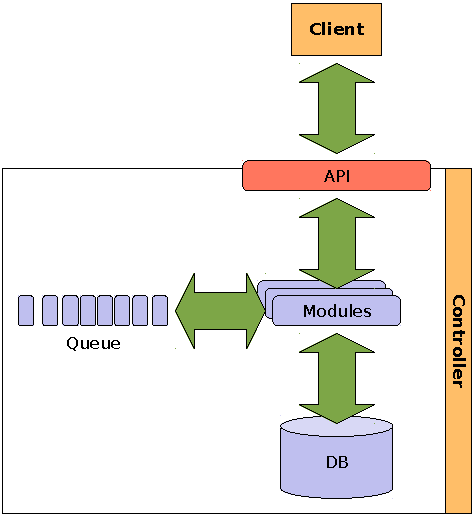
\includegraphics[width=0.5\textwidth]{imagenes/005.pdf}
 \caption{Cloud Controller in detail}
\label{fig:cloudcontroller}
\end{center}
\end{figure}

As a general rule, clients will interact with clouds through a Web Service API --- mostly \emph{RESTful} APIs (\emph{REpresentational State Transfer}). Those APIs vary slightly from company to vendor as usual, which forces clients to be partially coupled to clouds. That is why there has been an increasing trend for unifying and standardizing those APIs in order to guarantee compatibility inter-framework. Of special mention is the cloud standard proposed by the \emph{Open Grid Forum}: \emph{OCCI} (\emph{Open Cloud Computing Interface} \cite{occisdraft}).

The cloud's conforming modules support its functional requirements. Each one of them will have a well-defined responsibility, and so appear networking modules, access and security control modules, storage modules, etc. Many of them existed before the advent of Cloud Computing but they worked only locally. Inter-module communication is handled by means of an asynchronous message queue that guarantees an equally efficient broadcasting system outside of the Cloud Controller, i.e. the rest of the cluster nodes participating in the cloud.

To store and expose configuration data to the cluster in a single place while managing concurrent requests to update these data, every IaaS Framework evaluated resorts to a DBMS whose profiling must be properly tailored.

Hardware requirements on the cluster nodes vary from each particular framework implementation and the \emph{QoS} expected, but, in the abstract, they normally need something around 10 GB of RAM, quad core CPU, Gigabit Ethernet and one TB of storage.


\subsubsection{Cloud Node}\label{subsubsec:cloudnode}

\noindent If the Cloud Controller is entrusted the cloud's correct functioning acting like a glue for its parts, the actual task processing is performed in the Cloud Nodes; that is, the VCPU, VRAM, VHDD are going to be mapped from the corresponding CPU, RAM and HDD from the real nodes of the cluster.

Cloud Nodes may be heterogeneous according to their hardware characteristics. They will configure a resource set that, seen from the outside of the cluster, will appear to be a homogeneous whole where the summation of capacities of every participating node is the cloud's dimension. Further, this homogeneous space could be provisioned, as discussed above, on demand. It is the Cloud Controller's responsibility single out the optimal distribution of virtual servers throughout the cluster, attending to the physical aspects of both the virtual machine and the computer in which the former will run.

The most important subsystem in a Cloud Controller is the \emph{hypervisor} or \emph{VMM} (\emph{Virtual Machine Monitor}). The hypervisor is responsible for making possible the execution of virtual servers --- or virtual instances following the AWS nomenclature --- by creating the virtual architecture needed and a \emph{virtual execution domain} managed with the help of the operating system kernel. To generate this architecture there fundamentally exist three techniques: \emph{Emulation}, \emph{Paravirtualization} and \emph{Hardware Virtualization} or \emph{Full Virtualization}. Different hypervisors will support them in a different degree, but most will cover only one of them.

\subsection{Virtualization Techniques}\label{subsec:tecnicasemu}

\noindent What follows is a brief review of the main methods to create virtual infrastructure.

\subsubsection{Emulation}\label{subsubsec:emulacion}

\noindent Emulation is the most general virtualization method, in a sense that it does not call for anything special be present in the underlying hardware. However, it also carries the highest penalization in terms of performance. With emulation, every structure sustaining the virtual machine operation is created as a functional software copy of its hardware counterpart; i. e., every machine instruction to be executed in the virtual hardware must be run software-wise first, and then be translated on the fly into another machine instruction runnable in the physical domain --- the cluster node. The interpreter implementation and the divergence between emulated and real hardware will directly impact the translation overhead. This fact hinders the emulation from being widely employed in performance-critical deployments. Nonetheless, thanks to its operating flexibility it's generally used as a mechanism to support legacy systems. Besides, the kernel in the guest operating system --- the kernel in the virtual machines's --- operating system needs no alteration whatsoever, and the cluster node's kernel need only load a module.

\subsubsection{Hardware Virtualization}\label{subsubsec:virthardware}

\noindent Hardware Virtualization, on the contrary, allows host's processes to run directly atop the physical hardware layer, with no interpretation. Logically, this provides a considerable speedup from emulation, though imposes a special treatment to be given to its virtual processes. Regarding CPUs, both AMD's and Intel's support virtual process execution --- which is the capacity to run processes belonging to the virtual domain with little performance overhead --- as far as the convenient hardware extensions are present (\emph{SVM} and \emph{VT-x} respectively \cite{intelvtx}). Just as what happened with emulation, an unaltered host's kernel may be used. This fact is of relative importance as if wasn't so it would limit the myriad of OSs that could be installed as guests. Lastly, it should be pointed out that the hardware architecture is exposed to the VM as it is, i. e. with no software middleware.

\subsubsection{Paravirtualization}\label{subsubsec:paravirt}

\noindent Paravirtualization uses a different approach. To begin with, it is indispensable that the guest's kernel be modified to make it capable of interacting with a paravirtualized environment. When the guest runs, the hypervisor will separate those regions of instructions that have to be executed in kernel mode in the CPU, from those in user mode which will be executed as regular host processes. Subsequently, the hypervisor will manage an on-contract execution between host and guest allowing the latter to run kernel mode sections as if pertaining to the real execution domain --- as if they were processes running in the host, not in the guest --- with almost no performance slowdown. Paravirtualization, in turn, does not require an special hardware extension be present.

\subsection{Cloud IaaS frameworks}\label{subsec:frameworksiaas}

\noindent Cloud IaaS frameworks are those software systems managing the abstraction of complexity associated with on demand provisioning and administering failure-prone generic infrastructure. In spite of being almost all of them open sourced --- which fosters reusability and collaboration ---, they have evolved in different frames. This fact has raised a condition of lacking outwards interoperability, maturing non-standard APIs; though today those divergences are fading away. These frameworks and APIs are product of the efforts to improve and ease controlling the underlying particular clusters on which they germinated. Thus, it is no surprising their advances had originated parallelly with the infrastructure they drove, leaving compatibility in the background.

Slowly but steadily these managing systems became larger in reach and responsibility boosted by an increasingly interest in the sector. In the end, it happened that software and systems engineering made them more abstract, so they finally overlapped functionally. AWS appearance finished forging the latent standardization need, and thus, as of today, most frameworks offer APIs closer and closer to Amazon's --- nowadays the de-facto standard --- and OCCI's \cite{occisdraft}.

\section{MapReduce Paradigm}\label{sec:mapred}

\noindent The origin of the paradigm centers around a paper publication of two Google employees \cite{googlemapreduce}. In this paper they explained a method implementation devised to abstract the common parts present in distributed computing that rendered simple but large problems much more complex to solve when paralleling their execution on massive clusters. A concise definition states that MapReduce is ``\textit{a data processing model and execution environment that runs on large clusters of commodity computers}'' \cite{hadoopdefguide}.

\subsection{Programming Model}\label{subsec:programacionmapred}

\noindent The MapReduce programming model requires the developer express his problem as a partition of two well-defined pieces. A first part deals with the reading of input data and with producing a set of intermediate results that will be scattered over the cluster nodes. These intermediate transformations will be grouped according to an intermediate key value. A second phase begins with that grouping of intermediate results and concludes when every \emph{reduce} operation on the groupings succeeds. Seen from another vantage point, the first phase corresponds, broadly speaking, to the behavior of the functional \emph{map} and the second to the functional \emph{fold}.

In terms of the MapReduce model, these functional paradigm concepts give rise to \emph{Map} and \emph{Reduce} functions. Both Map and Reduce have to be supplied by the developer, which may force a deviation in breaking the original problem down. As counterpart, the MapReduce model will deal with parallelizing the computation, distributing input data across the cluster, handling exceptions that could raise and recovering output results; everything transparent to the programmer.

\subsubsection{Funci\'on Map}\label{map}

\noindent The typical functional map takes any function \texttt{F} and a list of elements \texttt{L} or, in general, any recursive data structure, to return a list resulting from applying \texttt{F} to each element of \texttt{L}. Figure \ref{fig:functionalmap} shows its signature and an example.

\begin{figure}[tbp]
\begin{center}
\begin{tabular}{|l|}
\hline
$\mathbf{map:} \: \left ( \alpha \rightarrow \beta \right ) \: \rightarrow \: \alpha \: list \: \rightarrow \: \beta \: list$ \\
$\mathbf{map} \: \left( \mathbf{pow}\:2 \right) \: \left[ 1,2,3 \right] \: \Rightarrow \: \left[ 1,4,9 \right ]$ \\
\hline
\end{tabular}
\caption{Map function example (functional version)}
\label{fig:functionalmap}
\end{center}
\end{figure}

In its MapReduce realization, map function receives a tuple as input and produces another tuple \texttt{(key, value)} as intermediate output. It is the MapReduce library who is responsible for feeding the map function by mutating the data contained in input files into \texttt{(key, value)} pairs. Then, it deals with grouping those intermediate tuples by key before passing them in as input to the reduce function. Input and output data types correspond to those shown in the function signature figure \ref{fig:mapreducemap}.

\begin{figure}[tbp]
\begin{center}
\begin{tabular}{|l|}
\hline
$\mathbf{map:} \: \left( k1,v1 \right) \: \rightarrow \: \left( k2,v2 \right) list$ \\
$\mathbf{k:} \: clave \linebreak$ \\
$\mathbf{v:} \: valor \linebreak$ \\
$\mathbf{\left(kn,vn \right):} \: par \: \left( clave,valor \right) \: en \: un \: dominio \: n$ \\
\hline
\end{tabular}
\caption{Map function signature (MapReduce version)}
\label{fig:mapreducemap}
\end{center}
\end{figure}


\subsubsection{Reduce function}\label{reduce}

\noindent The typical functional fold expects any function \texttt{G}, a list \texttt{L}, or generally any type of recursive data structure, and any initial element \texttt{I}, subtype of \texttt{L}'s elements. Fold returns the value in \texttt{I} resulting from building up the intermediate values generated after applying \texttt{G} to each element in \texttt{L}. Figure \ref{fig:fold} presents fold signature as well as an example.

\begin{figure}[tbp]
\begin{center}
\begin{tabular}{|l|}
\hline
$\mathbf{fold:} \: \left( \alpha \rightarrow \beta \rightarrow \alpha \right) \: \rightarrow \: \alpha \: \rightarrow \: \beta \: list \: \rightarrow \: \alpha$ \\
$\mathbf{fold} \: \left( \mathbf{+} \right) \: 0 \: \left[ 1,2,3 \right] \: \Rightarrow \: 6$ \\
\hline
\end{tabular}
\caption{Fold function example}
\label{fig:fold}
\end{center}
\end{figure}

Contrary to map, reduce expects the intermediate groups as input to produce a smaller set of values for each group as output, because reduce will iteratively \emph{fold} the groupings into values. Those reduced intermediate values will be passed in again to the reduce function if more values with the same key appeared from subsequent maps. Reduce signature is shown on figure \ref{fig:reduce}. Just as happens with map, MapReduce handles the transmission of intermediate results out from map into reduce. The model also describes the possibility to define a \emph{Combiner} function that would act after map partially reducing the values within the same grouping to lower network traffic --- the combiner usually runs in the same machine as the map.

\begin{figure}[tbp]
\begin{center}
\begin{tabular}{|l|}
\hline
$\mathbf{reduce:} \: \left( k2,v2 \: list \right) \: \rightarrow \: v2 \: list$ \\
$\mathbf{k:} \: clave$ \\
$\mathbf{v:} \: valor$ \\
$\mathbf{\left(kn,vn \right):} \: par \: \left(clave,valor\right) \: en \: un \: dominio \: n$ \\
\hline
\end{tabular}
\caption{Reduce function signature}
\label{fig:reduce}
\end{center}
\end{figure}

\subsubsection{A word counter in MapReduce}\label{subsubsec:wordcount}

\noindent As an example, figure \ref{fig:wordcount} shows the pseudocode of a MapReduce application to count the number of words in a document set.

\begin{figure}[tbp]
 \begin{center}
  \begin{tabular}{|l|}
   \hline
   \texttt{{\bf Map} (String key, String value):} \\
   \texttt{// key: documento name} \\
   \texttt{// value: document contents} \\
   \texttt{{\bf for each} word w {\bf in} value:} \\
   \texttt{{\bf EmitIntermediate} (w, ``1'')};\\ \\

   \texttt{{\bf Reduce} (String key, Iterator values):} \\
   \texttt{// key: a word} \\
   \texttt{// values: an Iterable over intermediate counts of the word key} \\
   \texttt{{\bf int} result = 0;} \\
   \texttt{{\bf for each} v {\bf in} values:} \\
   \texttt{{\bf Emit} ({\bf AsString} (result));} \\
   \hline
  \end{tabular}
  \caption{MapReduce wordcount pseudocode. Source: \cite{googlemapreduce}}
  \label{fig:wordcount}
 \end{center}
\end{figure}

In a wordcount execution flow the following is going to happen: map is going to be presented with a set of names containing all of the documents in plain text whose words will be counted. Map will subsequently iterate over each document in the set emitting the tuple \texttt{(<word>, ``1'')} for each word found. Thus, an explosion of intermediate pairs will be generated as output of map, will be distributed over the network and progressively folded in the reduce phase. Reduce is going to be input every pair generated by map but under a different form. Reduce will accept on each invocation the pair \texttt{(<word>, list(``1''))}. The list of \texttt{``1''}s, or generically an \texttt{Iterable} over \texttt{``1''}s, will contain as many elements as instances of the word \texttt{<word>} there were in the document set --- this supposing that the map phase were over before starting the reduce phase and that every word \texttt{<word>} were submitted to the same reducer in the cluster --- a cluster node executing the reduce function.

Once the flow had been completed, MapReduce would return a listing with every word in the documents and the number of times it appeared.

\subsection{Applicability of the Model}\label{subsec:aplicabilidad}

\noindent The myriad of problems that could be expressed following the MapReduce programming parading is clearly reflected in \cite{googlemapreduce}, a subset of them being:

\begin{itemize}
 \item Distributed grep: Map emits every line matching the regular expression. Reduce only forwards its input to its output acting as identity function.
 \item Count of URL access frequency: Like wordcount.
 \item Reverse web-link graph: For each URL contained in a web document, map generates the pair \texttt{(<target_URL>, <source_URL>)}. Reduce will emit the pair \texttt{(target, list(source))}.
 \item Inverted index: Map parses each document and emits a series of tuples in the form \texttt{(<word>, <document_id>)}. All of them are passed as input to reduce that generates the sequence of pairs \texttt{(<word>, list(document_id))}.
\end{itemize}

\subsection{Processing Model}\label{subsec:processingmodel}

\noindent Besides defining the structure that the applications willing to leverage the MapReduce capabilities will have to follow --- so that they need not code their own distribution mechanisms ---, with \cite{googlemapreduce} an implementation of the model was introduced which allowed Google to stay protocol, architecture and system agnostic while keeping their commodity clusters on full utilization. This agnosticism allows for deploying vendor-lock-free distributed systems.

The MapReduce model works by receiving self-contained processing requests called \emph{job}s. Each job is a \emph{partition} of smaller duties called \emph{task}s. A job won't be completed until no task is pending for finishing execution. The processing model main intent is to distribute the tasks throughout the cluster in a way that reduced job latency. In general, it can be stated that task processing on each phase is done in parallel and phases execute in sequence; yet, it is not needed for reduce to wait until map is complete.

Figure \ref{fig:exmapreduce} shows a summary of a typical execution flow. It is interesting enough to deepen in its details as many other MapReduce implementations will present similar approaches.

\begin{figure}[tbp]
\begin{center}
 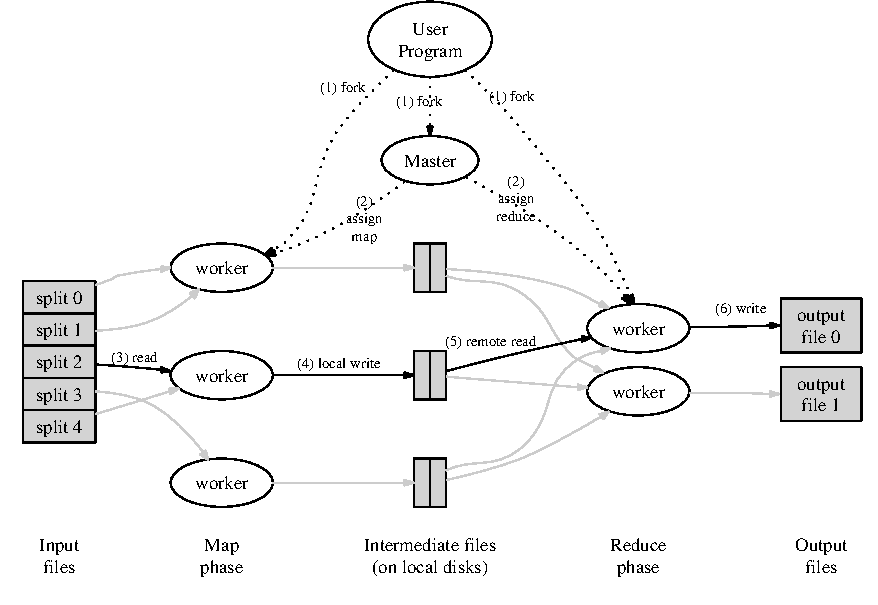
\includegraphics[width=0.9\textwidth]{imagenes/006.pdf}
 \caption{MapReduce execution diagram. Source: \cite{googlemapreduce}}
 \label{fig:exmapreduce}
\end{center}
\end{figure}

\begin{enumerate}
 \item MapReduce divides input files in \texttt{M} parts, the size of which is parameterized, and distributes as many copies of the MapReduce user algorithm as nodes participate in the computation.
 \item From this moment each program copy resides in a cluster node. A random copy is chosen among them and labeled as the \emph{Master Replica}, effectively assigning the \emph{Master Role} to the node holding the replica; every other node in the cluster is designated with the \emph{Slave Role}. Those slave nodes will receive the actual MapReduce tasks and their execution will be driven from the master node. There will be \texttt{M} map tasks and \texttt{R} reduce tasks
 \item 
\end{enumerate}

\begin{enumerate}
 \item MapReduce divide los ficheros de entrada en \emph{M} partes, de tama\~no configurable usando un par\'ametro, y distribuye tantas copias del programa del usuario ---t\'ipicamente s\'olo las implementaciones concretas de Map y Reduce--- como nodos participen en la computaci\'on.
 \item Ahora cada copia del programa reside en un nodo. Se define entonces que una de esas copias sea especial ---la r\'eplica \emph{Master}--- de forma que el resto quedan residiendo en nodos que, en adelante, son considerados \emph{trabajadores} o \emph{esclavos}. O dicho de otro modo, desde el momento en que se nombra la copia maestra, se determina el rol \emph{maestro} del cl\'uster, que recae sobre el nodo que posee la copia maestra; los dem\'as nodos tendr\'an en su poder copias no maestras o esclavas, fijando, igualmente, su rol a esclavos. Estos nodos esclavos son los que reciben las tareas concretas de ejecuci\'on dirigidos por el maestro. Habr\'a \emph{M} tareas Map y \emph{R} tareas Reduce que el maestro ha de repartir entre sus trabajadores inactivos y que podr\'an ser procesadas en paralelo.
 \item Los trabajadores a los que se les hayan asignado tareas Map leen las porciones de los ficheros de entrada correspondientes, \emph{parsean} los do\-cu\-men\-tos generando pares \texttt{(clave, valor)} que redirigen a la funci\'on Map del usuario. El contenido de salida de Map se mantiene en memoria a modo de b\'uffer.
 \item Peri\'odicamente, esos pares en memoria son volcados a \emph{disco local} y particionados en \emph{R} regiones. Su posici\'on en disco es enviada al maestro, responsable de informar de la localizaci\'on de esos pares intermedios a los trabajadores con tareas Reduce.
 \item En el momento en que un trabajador Reduce es notificado de que sus datos de ejecuci\'on, esto es, los datos de una partici\'on que le co\-rres\-pon\-de, est\'an disponibles, \'este lee la informaci\'on del disco del trabajador Map a trav\'es de \emph{RPC} (\emph{Remote Procedure Call}) y, antes de invocar la funci\'on Reduce del usuario, ordena los pares intermedios por clave.
 \item Finalmente, el trabajador Reduce itera sobre los pares ordenados por clave, enviando, a la funci\'on Reduce del usuario, la clave y el conjunto de valores asociados a esa clave. La salida de la funci\'on Reduce para esa partici\'on se va escribiendo en un archivo de salida sobre el sistema de ficheros distribuido.
\end{enumerate}

Cuando se hayan completado todas las tareas Map y Reduce, el espacio particionado de salida ---los ficheros de salida de cada partici\'on--- se env\'ia al programa que haya hecho la llamada a MapReduce.
El modelo de ejecuci\'on es lo suficientemente gen\'erico como para aplicarse a la resoluci\'on de problemas de distinto tama\~no, corriendo sobre clusters indeterminadamente grandes.


\subsection{Tolerancia a fallo}\label{subsec:toleranciafallos}
\noindent La idea de proporcionar un marco de ejecuci\'on de trabajos lo suficientemente grandes como para necesitar enormes conjuntos de m\'aquinas de procesado para mantener los tiempos de latencia en valores razonables, pasa, forzosamente, por definir una pol\'itica que asegure cierta resistencia a unos fallos que seguramente aparecer\'an. De no ser considerados, estos fallos derivar\'ian en errores de distinto grado de severidad: unos provocar\'ian que se perdiesen tareas ya completadas, otros, menos problem\'aticos, inhibir\'ian los datos intermedios, siendo improbable la conclusi\'on con \'exito de la ejecuci\'on. Sea como fuere, el propio modelo MapReduce prevee una serie de problemas en el procesamiento e implementa una serie de actuaciones ante cada uno de ellos.


\subsubsection{Fallo en trabajador}\label{subsubsec:fallotrabajador}
\noindent El menos problem\'atico. Para controlar que todos los trabajadores al cargo de un maestro funcionan correctamente, cada cierto tiempo el maestro env\'ia una petici\'on de respuesta de eco ---el cl\'asico \emph{ping}--- a todos estos trabajadores. Si alguno de ellos no contestase de forma reiterada, \'este quedar\'ia registrado en el maestro como \emph{inaccesible}.\newline

Un trabajador marcado inaccesible no recibir\'a nuevas tareas, ni tampoco podr\'a ser accedido remotamente por los trabajadores Reduce para cargar los resultados de sus Map intermedios, lo que puede suponer un problema insalvable para completar la ejecuci\'on. El acceso a estos datos intermedios se resuelve marcando, de nuevo en el maestro, las tareas asignadas al trabajador ca\'ido como \emph{inactivas}. As\'i, \'estas ser\'an programadas para ser procesadas de nuevo en alg\'un trabajador activo, que colocar\'a los resultados intermedios en alg\'un punto accesible por los nodos Reduce. Adem\'as, en el momento de detectar la incapacidad operativa de un trabajador, el maestro informar\'a de este hecho al resto de trabajadores esclavos para evitar, por ejemplo, errores en la lectura de los datos intermedios.


\subsubsection{Fallo en maestro}\label{subsubsec:fallomaestro}
\noindent El fallo en el nodo maestro es el m\'as problem\'atico. La aproximaci\'on propuesta consiste en ordenar que el maestro cree peri\'odicamente puntos de restauraci\'on desde los que pueda reanudar su ejecuci\'on en caso de que se terminase inesperadamente. Ya que el maestro es \'unico, la probabilidad de fallo es mucho menor que para el caso general de fallo en un nodo; de hecho, lo suficientemente baja como para que se proponga en \cite{googlemapreduce} que se aborte la ejecuci\'on del trabajo al completo si el maestro fallase. Como primera soluci\'on es acep\-ta\-ble. No obstante, dado que no tiene ning\'un sentido dejar un \emph{punto de fallo singular} f\'acil de abordar al descubierto, frameworks posteriores proponen replicar el comportamiento del maestro en otros nodos.


\subsection{Caracter\'isticas adicionales}\label{subsec:caracteristicasadicionales}
\noindent A continuaci\'on se resumen otras cuestiones adicionales estudiadas para este framework MapReduce.

\subsubsection{Localidad}\label{subsubsec:localidad}
\noindent El cuello de botella en un despliegue t\'ipico es el ancho de banda de red. En una ejecuci\'on cualquiera, la informaci\'on se propaga desde el cliente hacia el sistema de ficheros distribuido del cl\'uster MapReduce. Como se ha comentado, cada nodo posee una cierta capacidad de almacenamiento y ejecuci\'on de tareas sobre los datos de entrada. De esta forma, cada paso del procesado global requiere la transmisi\'on por la red de enormes cantidades de informaci\'on ---recordar, por ejemplo, la E/S de la funci\'on Map en wordcount--- colapsando r\'apidamente su ancho de banda y limitando, por tanto, la velocidad de ejecuci\'on. Para mitigar este problema, se afina el sistema de ficheros distribuido para que aproxime la informaci\'on al nodo del cl\'uster que ha de procesar esa informaci\'on, reduciendo considerablemente las transferencias acometidas para completar los trabajos, minimizando as\'i el tr\'afico de red requerido.


\subsubsection{Complejidad}\label{subsubsec:complejidad}
\noindent A priori, las variables \emph{M} y \emph{R} de las ejecuciones MapReduce ---recordemos, la dimensi\'on de las particiones del espacio de entrada e intermedio res\-pec\-ti\-va\-men\-te--- pueden tomar valores cualesquiera configurables por el usuario. Sin embargo, existen ciertos l\'imites pr\'acticos. Por cada trabajo MapReduce que se est\'e gestionando, el maestro ha de hacer $O(M + R)$ decisiones de planificaci\'on ---suponiendo que no se produjese ning\'un error que forzase replanificar tareas--- ya que cada partici\'on del espacio de entrada, \emph{M}, habr\'a de repartirse entre los trabajadores Map, y cada partici\'on del espacio de salida de Map, \emph{R}, entre los trabajadores Reduce; de ah\'i la expresi\'on de la \emph{complejidad temporal}. En cuanto a la \emph{complejidad espacial}, el maestro tendr\'a que mantener $O(M \cdot R)$ de memoria de estado. La expresi\'on se optiene al razonar que, en el peor de los casos, cada parte del fichero de entrada se mapear\'a sobre cada parte del espacio intermedio.


\subsubsection{Tareas secundarias}\label{subsubsec:secundarias}
\noindent Podr\'ia caber la situaci\'on en la que un nodo del cl\'uster estuviese ejecutando tareas Map o Reduce a una velocidad m\'as lenta de lo habitual; por ejemplo, si tuviese el disco r\'igido da\~nado, las lecturas y escrituras se suceder\'ian m\'as lentamente, y como el trabajo MapReduce no est\'a completado hasta que todas sus tareas componentes hayan finalizado con \'exito, el nodo problem\'atico estar\'ia ocasionando una limitaci\'on en el rendimiento global. Para aliviar el problema, se propone que cuando falte por concluir la ejecuci\'on de pocas ta\-re\-as del trabajo, \'estas sean enviadas a dos nodos trabajadores: una como tarea convencional y otra como tarea secundaria de alg\'un nodo inactivo. En el momento en que concluya la ejecuci\'on de alguna de las dos, esa tarea se marcar\'a como terminada, reduciendo la latencia que a\~naden esos nodos con dificultades operativas.


\subsubsection{Funci\'on Combiner}\label{subsubsec:combiner}
\noindent En muchas ocasiones sucede que existe un gran n\'umero de pares intermedios generados que se repiten. Tomando como ejemplo el wordcount expuesto antes, se puede deducir que cada trabajador Map generar\'a ingentes cantidades de registros de la forma \texttt{(``a'', ``1'')}, que ser\'an enviados por la red hacia los trabajadores Reduce. Un mecanismo para reducir este colapso es permitir al usuario escribir una funci\'on de combinaci\'on de resultados intermedios, que se lanzar\'a previa ejecuci\'on de la funci\'on Reduce. Esta funci\'on combinadora ir\'a recogiendo los resultados intermedios, dentro del mismo trabajador Map, para hacer una primera reducci\'on (o combinaci\'on) de los datos antes de ser marcados como disponibles para los trabajadores Reduce.\newline

T\'ipicamente, el c\'odigo fuente de ambas funciones ---Reduce y Combiner--- es el mismo; lo que s\'i cambia es el modo en que la librer\'ia MapReduce gestiona su ejecuci\'on: la salida de la combinaci\'on se mantiene en disco local y no en el sistema de ficheros distribuido, para reducir la sobrecarga de red que supondr\'ia.


\subsection{Frameworks MapReduce}\label{subsec:frameworksmapred}
\noindent Desde 2004 han ido apareciendo multitud de frameworks que codifican, considerando distintas optimizaciones, la funcionalidad del paradigma. Por citar algunos nombres:

\begin{description}
 \item[Hadoop] \cite{hadoopdefguide} Uno de los primeros en cubrir el modelo de procesado pro\-pues\-to para MapReduce y principal implementaci\'on de referencia para los dem\'as frameworks. Es el m\'as utilizado, probado y desplegado con diferencia en la actualidad.
 \item[GridGain] \cite{gridgainvshadoop} Comercial y centrado en el procesado en memoria para ace\-le\-rar la ejecuci\'on: menor latencia de acceso al dato a costa de un menor espacio de E/S.
 \item[Twister] \cite{twister} Desarrollado como proyecto de investigaci\'on en la Universidad de Indiana, pretende dar un giro de tuerca m\'as al modelo MapReduce, abstrayendo las partes comunes y necesarias para lanzar ejecuciones, aisl\'andolas y almacen\'andolas en memoria distribuida como objetos est\'aticos, reduciendo as\'i el tiempo necesario para configurar las funciones Map y Reduce previo procesado.
 \item[GATK] \cite{gatk} Utilizado en investifaci\'on gen\'etica para evaluar y secuenciar fragmentos de ADN de m\'ultiples especies.
 \item[Qizmt] \cite{qizmt} Escrito en C\# y puesto en funcionamiento para MySpace.
 \item[misco] \cite{misco} Escrito 100\% en Python y basado en trabajos previos de Nokia, se propone como implementaci\'on MapReduce capaz de correr en dispositivos m\'oviles.
 \item[Peregrine] \cite{peregrine} Optimizando el modo en que se manipulan los resultados intermedios y pasando toda operaci\'on de E/S a una cola as\'incrona, entre otras alteraciones, han llegado a acelerar bastante la ejecuci\'on de tareas. Todav\'ia en beta a junio de 2013.
 \item[Mars] \cite{mars} Implementado en \emph{NVIDIA CUDA}, se centra en extraer el m\'aximo rendimiento de mapeo y reducci\'on moviendo la operativa a la tarjeta gr\'afica. En seis pruebas realizadas con Mars se han observado incrementos de rendimiento superiores a un orden de magnitud frente a ejecuciones en CPU.

\end{description}

De todos ellos Hadoop es, incuestionablemente, el framework MapReduce m\'as utilizado en la actualidad. Su naturaleza de c\'odigo abierto y su flexibilidad, tanto de procesado como de almacenamiento, le han reportado un creciente inter\'es desde la industria de la IT, que se ha venido traduciendo en la aparici\'on de numerosas herramientas acoplables a Hadoop que extienden su funcionalidad.


